\documentclass{article}

% Language setting
% Replace `english' with e.g. `spanish' to change the document language
\usepackage[english]{babel}

% Set page size and margins
% Replace `letterpaper' with `a4paper' for UK/EU standard size
\usepackage[letterpaper,top=2cm,bottom=2cm,left=3cm,right=3cm,marginparwidth=1.75cm]{geometry}

% Useful packages
\usepackage{amsmath}
\usepackage{graphicx}
\usepackage[colorlinks=true, allcolors=blue]{hyperref}

\title{Project Report}
\author{Andy Martinez and Daniel Sun-Friedman}

\begin{document}
\maketitle

\section{Section 1: Analytical Analysis}

The standard algorithm simply multiplies the two matrices using arithmetic operations. It calculates a total of $n^2$ entries, and to calculate each entry, it does $n$ separate multiplications of pairs of elements, and then sums them all up with $n-1$ additions. Thus, each element takes $n+(n-1)=2n-1$ time to calculate (based on the assumption that all arithmetic operations run in $O(1)$ time), so the amount of time to calculate the entire matrix product is $$T(n)=n^2(2n-1).$$

We learned in lecture that the runtime for Strassen's algorithm is $$T(n)=7T\left(\frac{n}{2}\right) + \Theta(n^2).$$

When we examine the algorithm we find that the exact value is $$T(n)=7T\left(\frac{n}{2}\right) + 18\left(\frac{n}{2}\right)^2,$$ since there are 18 places where the algorithm adds or subtracts matrices, and all of these matrices are of size $\left(\frac{n}{2}\right)^2$. However, there is one more technicality we must account for to obtain the correct runtime for Strassen's algorithm. Namely, if $n$ is odd, we cannot simply split it into matrices of size $\left(\frac{n}{2}\right)^2$. Instead, we can pad both matrices with an extra row and an extra column of zeroes (which takes constant runtime), so that the matrices are of even length. Then, we can write our equation in terms of $\frac{n+1}{2}$ instead of $\frac{n}{2}$: $$T(n)=7T\left(\frac{n+1}{2}\right) + 18\left(\frac{n+1}{2}\right)^2.$$

Let us first examine the even case. At the turning point, we will be using the conventional algorithm to calculate our matrix products of size $\frac{n}{2}$. Therefore, we will plug $\frac{n}{2}$ into our initial equation for the conventional algorithm's runtime: $$T\left(\frac{n}{2}\right) = \left(\frac{n}{2}\right)^2*\left(2\left(\frac{n}{2}\right)-1\right).$$

Thus we find that $$T(n)=7T\left(\frac{n}{2}\right) + 18\left(\frac{n}{2}\right)^2$$ $$= 7\left(\left(\frac{n}{2}\right)^2*\left(2\left(\frac{n}{2}\right)-1\right)\right) + 18\left(\frac{n}{2}\right)^2$$ $$= \frac{7}{4}n^2(n-1) + \frac{18}{4}n^2$$ $$= \frac{7}{4}n^3 - \frac{7}{4}n^2 + \frac{18}{4}n^2$$ $$= \frac{7}{4}n^3 + \frac{11}{4}n^2.$$


From here, we can also consider the fact that at the turning point, running Strassen's algorithm and running the conventional algorithm should take approximately the same amount of time. Therefore, it must also be the case that $$T(n)=n^2(2n-1).$$

Thus, we get that $$n^2(2n-1) = T(n) = \frac{7}{4}n^3 + \frac{11}{4}n^2$$ $$\implies \frac{7}{4}n^3 + \frac{11}{4}n^2 - n^2(2n-1) = 0$$ $$\implies \frac{7}{4}n^3 + \frac{11}{4}n^2 - n^2(2n-1) = \frac{7}{4}n^3 + \frac{11}{4}n^2 - 2n^3 + n^2$$ $$=-\frac{1}{4}n^3+\frac{15}{4}n^2=-\frac{1}{4}n^2(n-15) = 0$$ $$\implies n-15=0 \implies n = 15.$$

Thus, in the even case, $n=15$. (Note that $n=0$ also satisfies our equation, but it is not the answer we are looking for since the turning point cannot be at $n=0$.)

\medskip

Now we will examine the odd case. We start by once again using the standard algorithm runtime on our subcase, but this time we plug $\frac{n+1}{2}$ into this algorithm to get $$T\left(\frac{n+1}{2}\right) = \left(\frac{n+1}{2}\right)^2*\left(2\left(\frac{n+1}{2}\right)-1\right).$$

Thus, we have that $$T(n)=7T\left(\frac{n+1}{2}\right) + 18\left(\frac{n+1}{2}\right)^2$$ $$= 7\left(\left(\frac{n+1}{2}\right)^2*\left(2\left(\frac{n+1}{2}\right)-1\right)\right) + 18\left(\frac{n+1}{2}\right)^2$$ $$=\frac{7}{4}(n+1)^2(n) + \frac{18}{4}((n+1)^2)$$ $$= \left(\frac{7}{4}n +\frac{18}{4} \right)(n^2+2n+1)$$ $$= \frac{7}{4}n^3 + \frac{14}{4}n^2 + \frac{7}{4}n +\frac{18}{4}n^2 + \frac{36}{4}n + \frac{18}{4}$$ $$=\frac{7}{4}n^3 + 8n^2 + \frac{43}{4}n + \frac{9}{2}.$$

Once again, we remember that at the turning point, running Strassen's algorithm and running the conventional algorithm should take approximately the same amount of time. Thus, $$T(n)=n^2(2n-1).$$

This implies that $$n^2(2n-1) = T(n) = \frac{7}{4}n^3 + 8n^2 + \frac{43}{4}n + \frac{9}{2}$$ $$\implies \frac{7}{4}n^3 + 8n^2 + \frac{43}{4}n + \frac{9}{2} - n^2(2n-1) = 0$$ $$ \implies \frac{7}{4}n^3 + 8n^2 + \frac{43}{4}n + \frac{9}{2} - n^2(2n-1) =  \frac{7}{4}n^3 + 8n^2 + \frac{43}{4}n + \frac{9}{2} - 2n^3 + n^2$$ $$= -\frac{1}{4}n^3 + 9n^2 + \frac{43}{4}n + \frac{9}{2}$$ $$= -\frac{1}{4}(n^3 - 36n^2 - 43n - 18) = 0.$$

When we plug this function into Desmos, we find that the value of $n$ that satisfies the equation is approximately $n=37$, as shown in the image below. (Note that this image graphs our expression without the constant of $-\frac{1}{4}$, since omitting this constant does not change where the zeroes are.) 

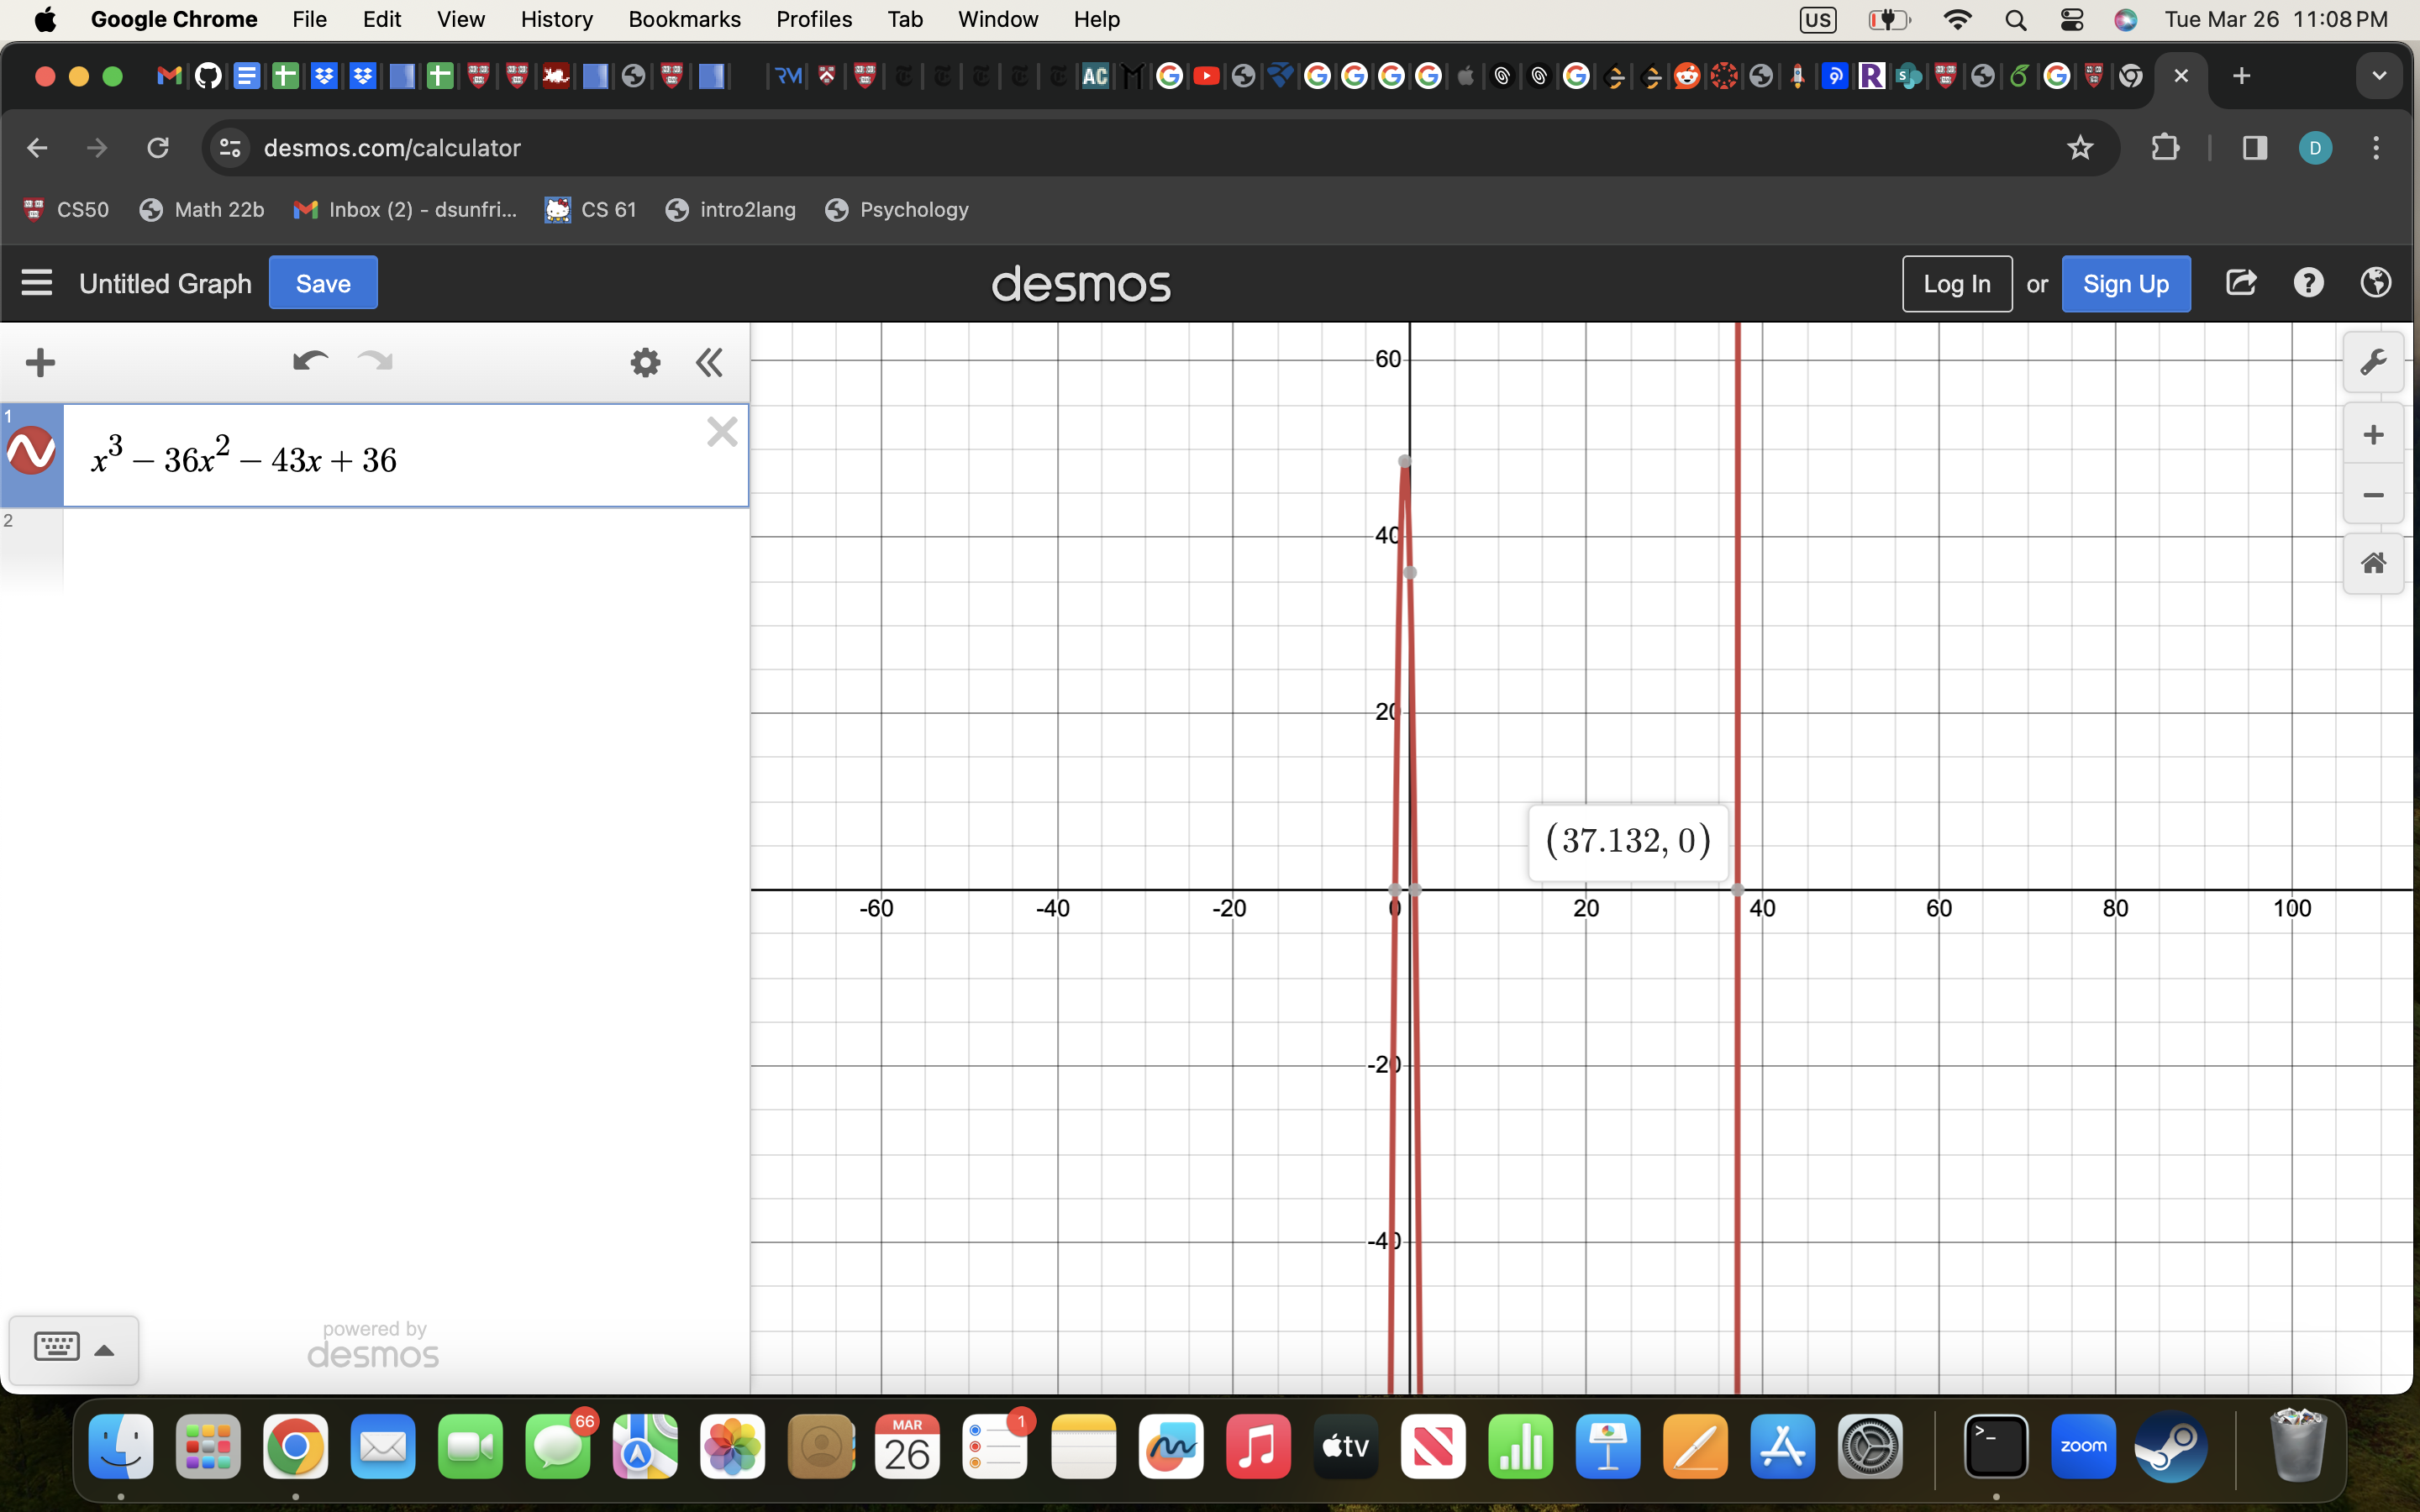
\includegraphics[width=\linewidth]{StrassenPlot.png}

Thus, our final result is that for the even case, the turning point is at $n=15$, and for the odd case, the turning point is at approximately $n=37$.

\pagebreak

\section{Section 2: Experimental Analysis}
After implementing the Strassen's algorithm, in a way that works for all n values, we can use a the time python package to empirically figure out the best n value or a range of optimal n values. In this case, I ran Strassen's algorithm on square matrices with the following dimensions [2, 4, 8, 16, 32, 64, 128, 256]. For each matrix I ran Strassen's algorithm with the following base values [1, 2, 3, 4, 5, 6, 7, 8, 9, 10, 15, 20, 32, 50, 100, 150] and got the following graph.

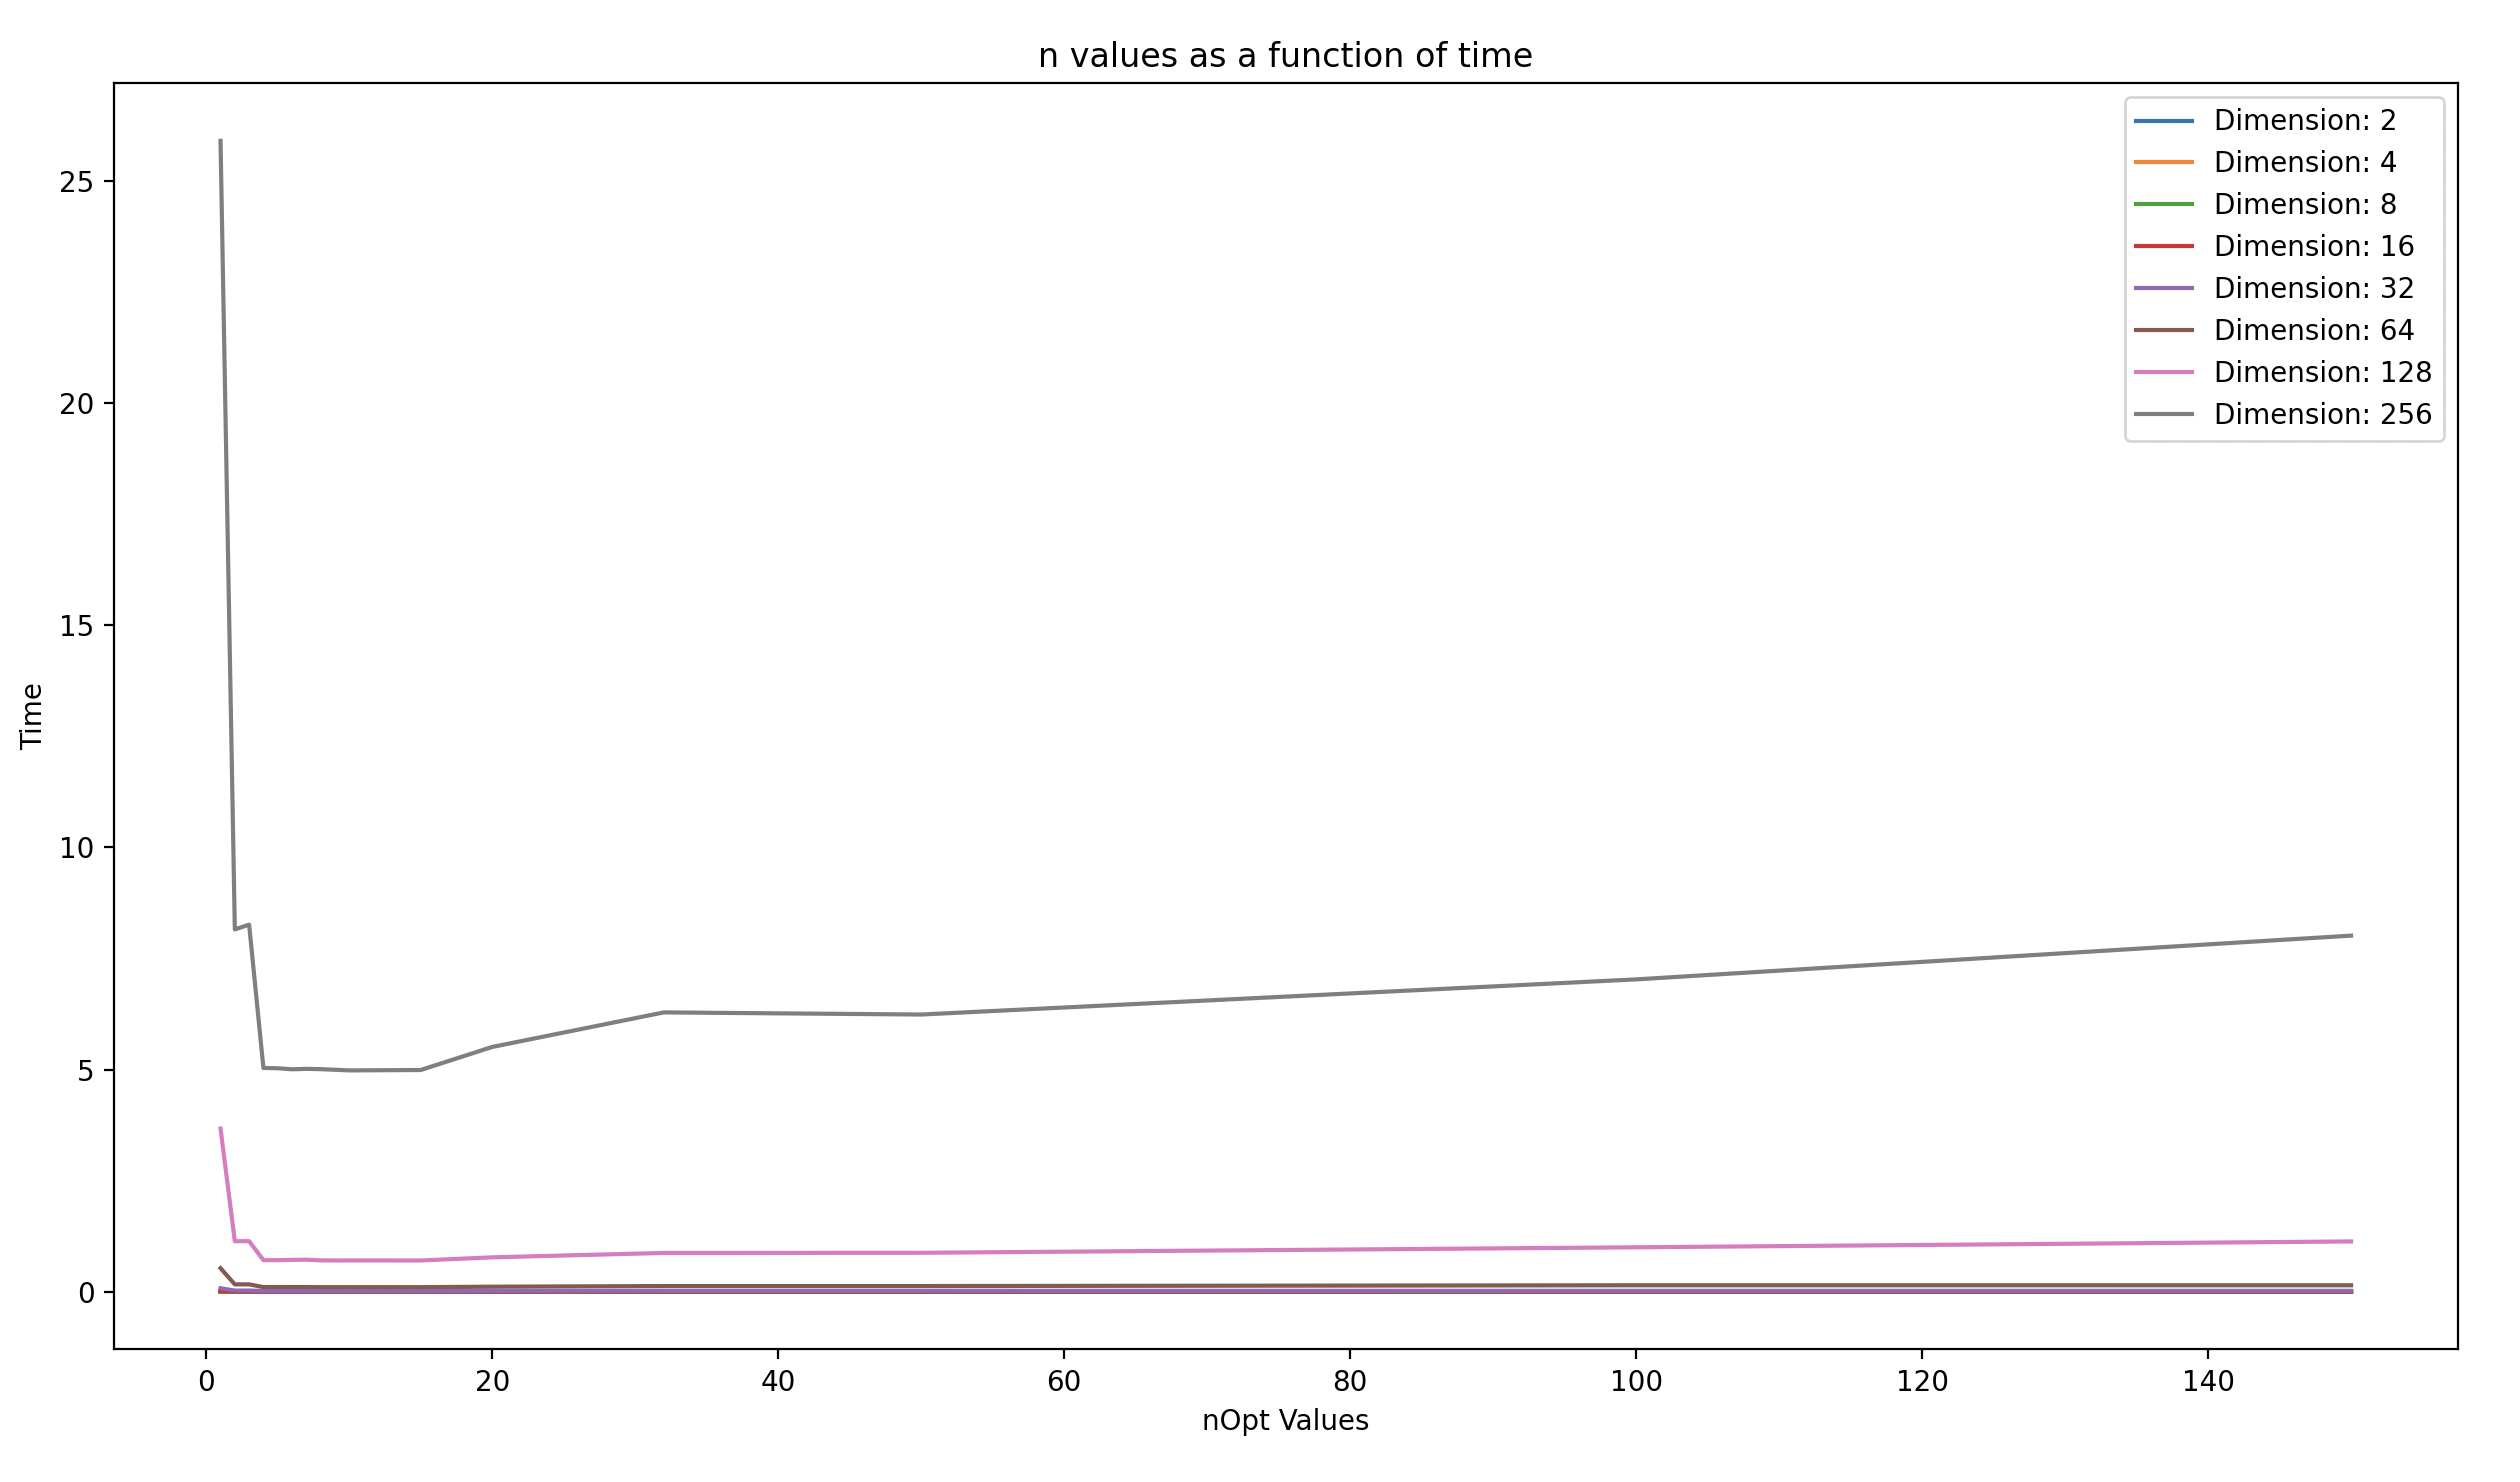
\includegraphics[width=\textwidth]{graph.png} \\

As we can see in the graph, the optimal size of the base case value seems to be in the range of 5 to around 15. The time values within this range tend to be very close together so any one of these values could be the optimal size to stop the base case. With that being said, according to the test that I ran, a base case n value of n = 9 seemed to get the best times across the board.

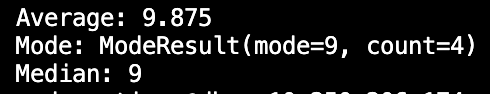
\includegraphics[width=\textwidth]{best_n.png} \\

In summary, according to my trials, any value from between 5 - 15 should give the optimal base case value for Strassen's algorithm, but 9 is the best according to my testing. Now, to find the cross-over point. I will run the algorithm twice, once using the traditional base case of a 1x1 matrix and another using the optimal base case found in the first part. Below are two graphs, one is zoomed in for lower dimensional values and the second one is zoomed out.

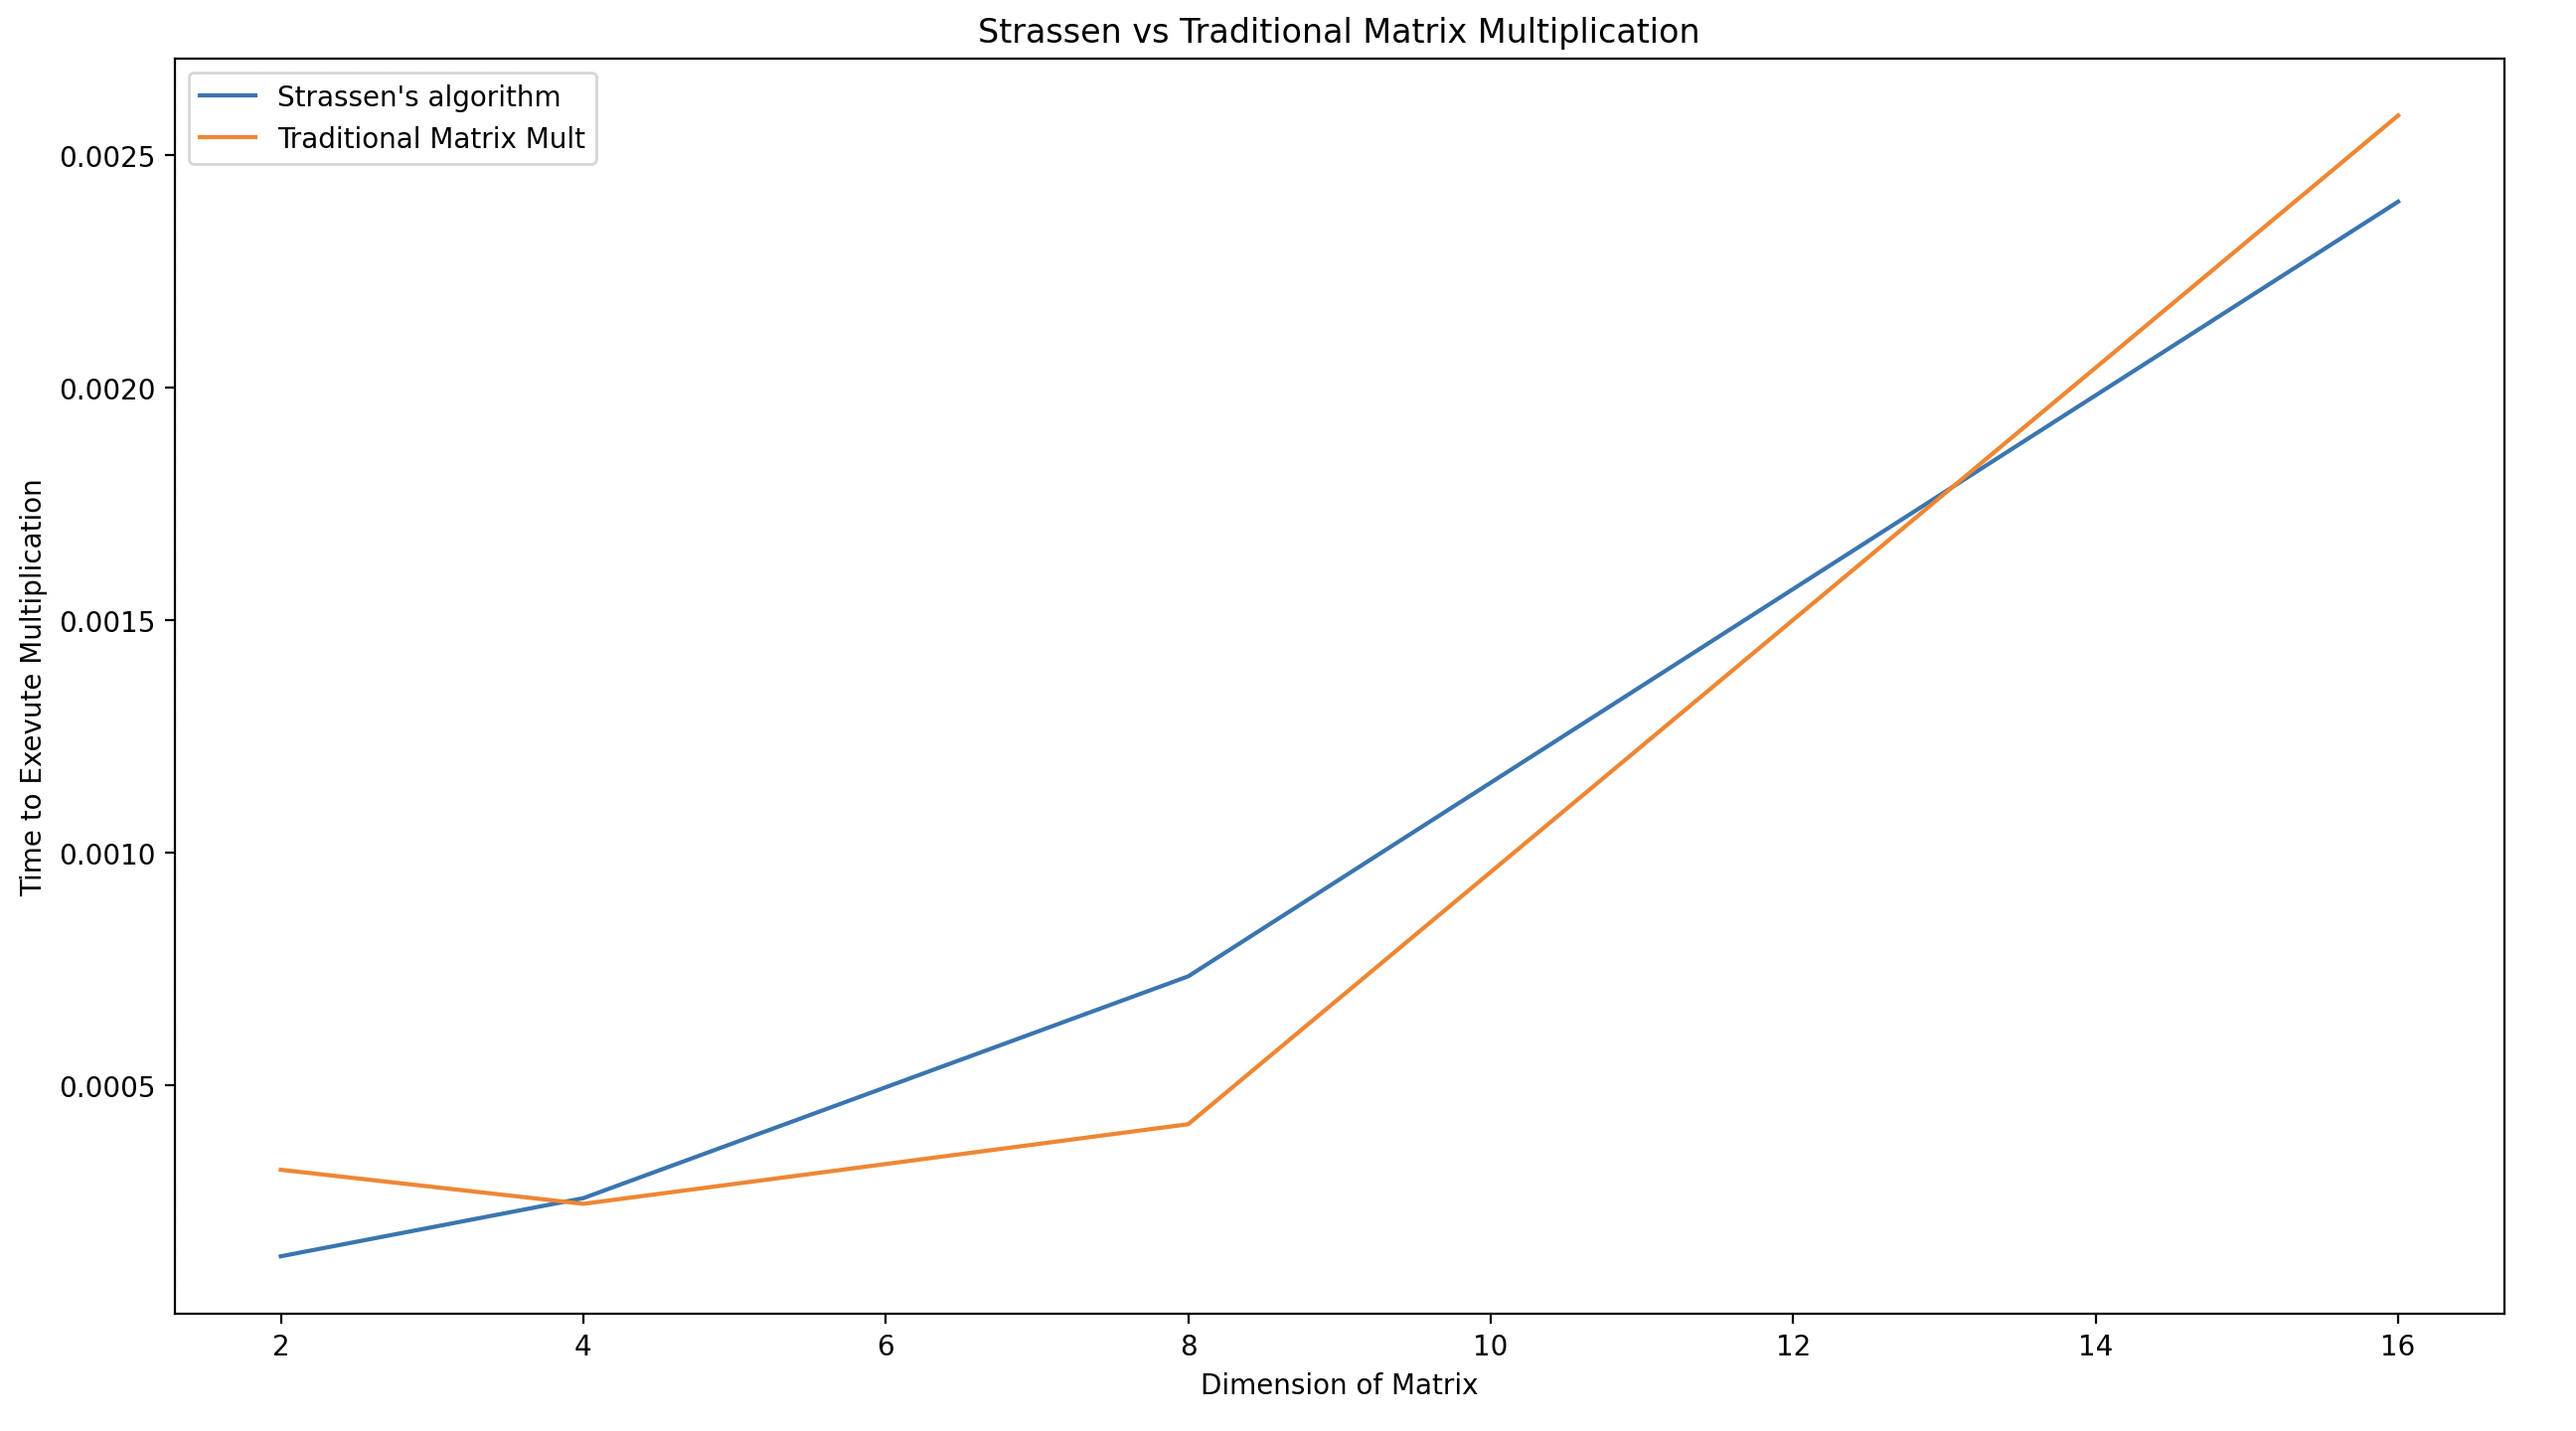
\includegraphics[width=\textwidth]{graph2.png}
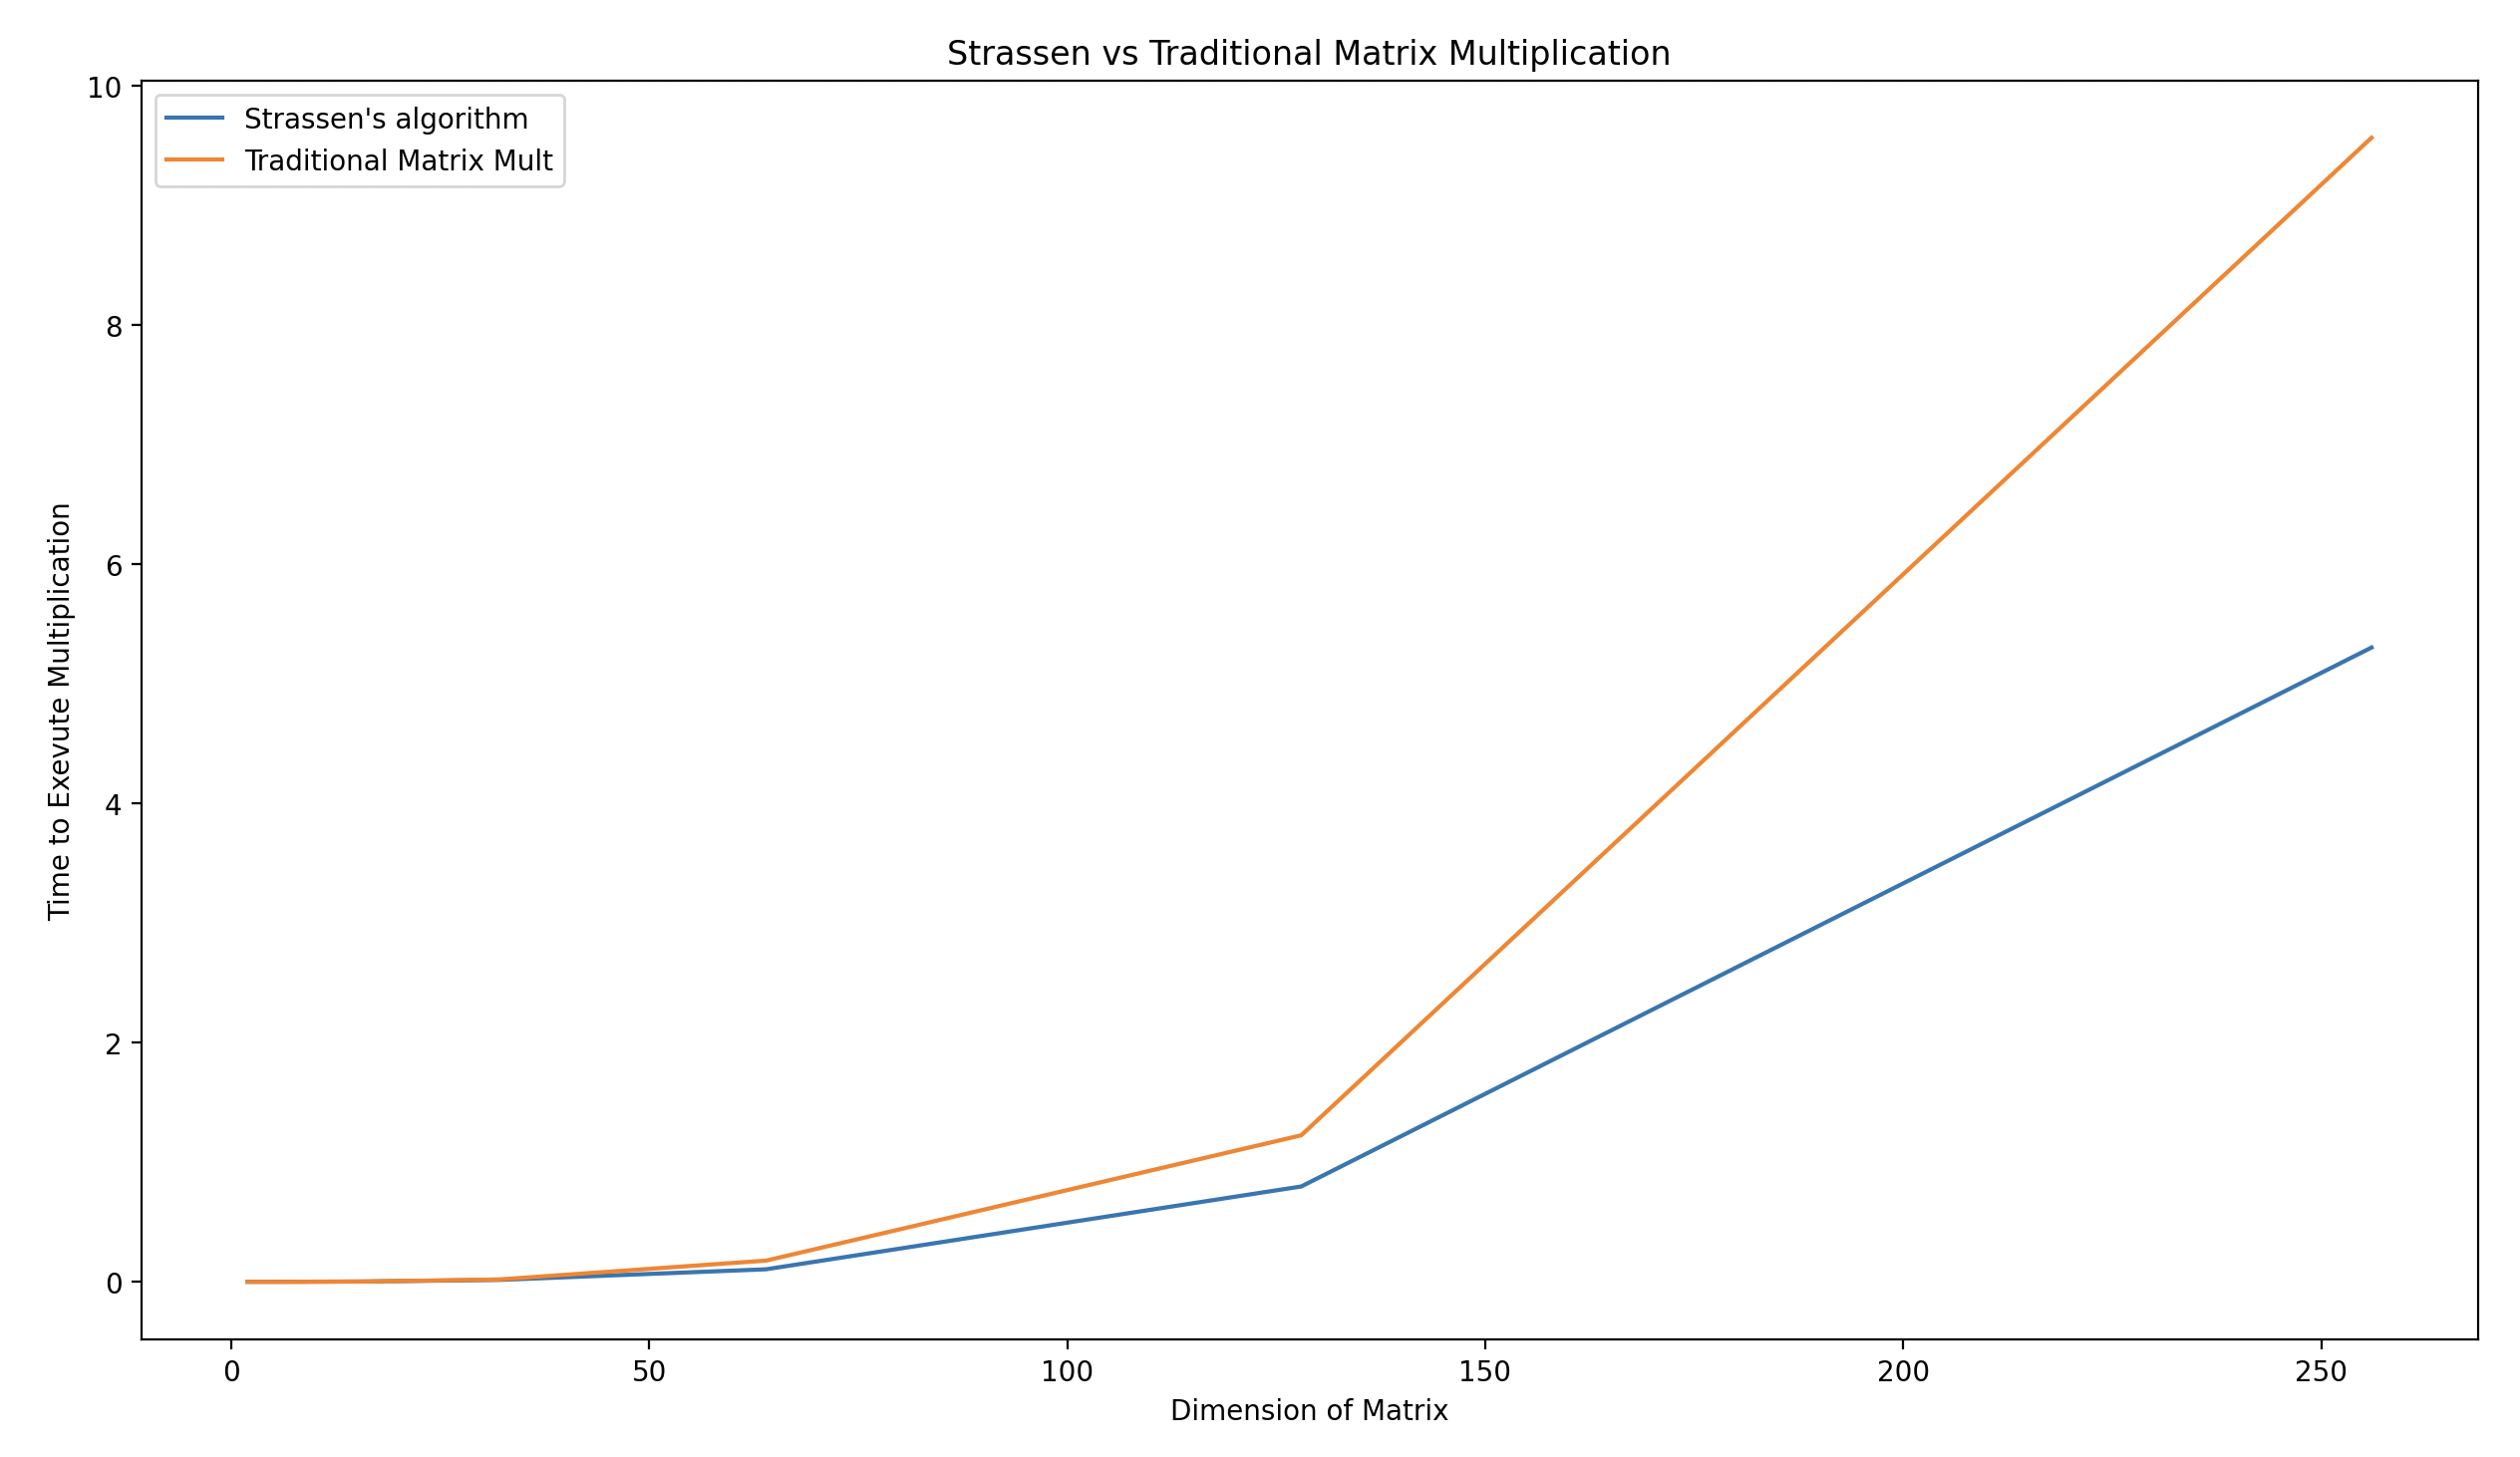
\includegraphics[width=\textwidth]{graph3.png} \\

In this case, we see the two methods are pretty much equal for smaller values, this makes sense seeing as this is Strassen's with a base case of 9. Thus, for values less than of equal to 9 dimensions, the two are essentially idential algorithms. With this optimized Strassen's we see that the cross over point happens at around n = 13. However, with the optimized Strassen's is pretty much always better than the traditional method of conducting matrix multiplication. Now, let's compare it to the Strassen's matrix multiplication with the normal base case of a 1x1 matrix.

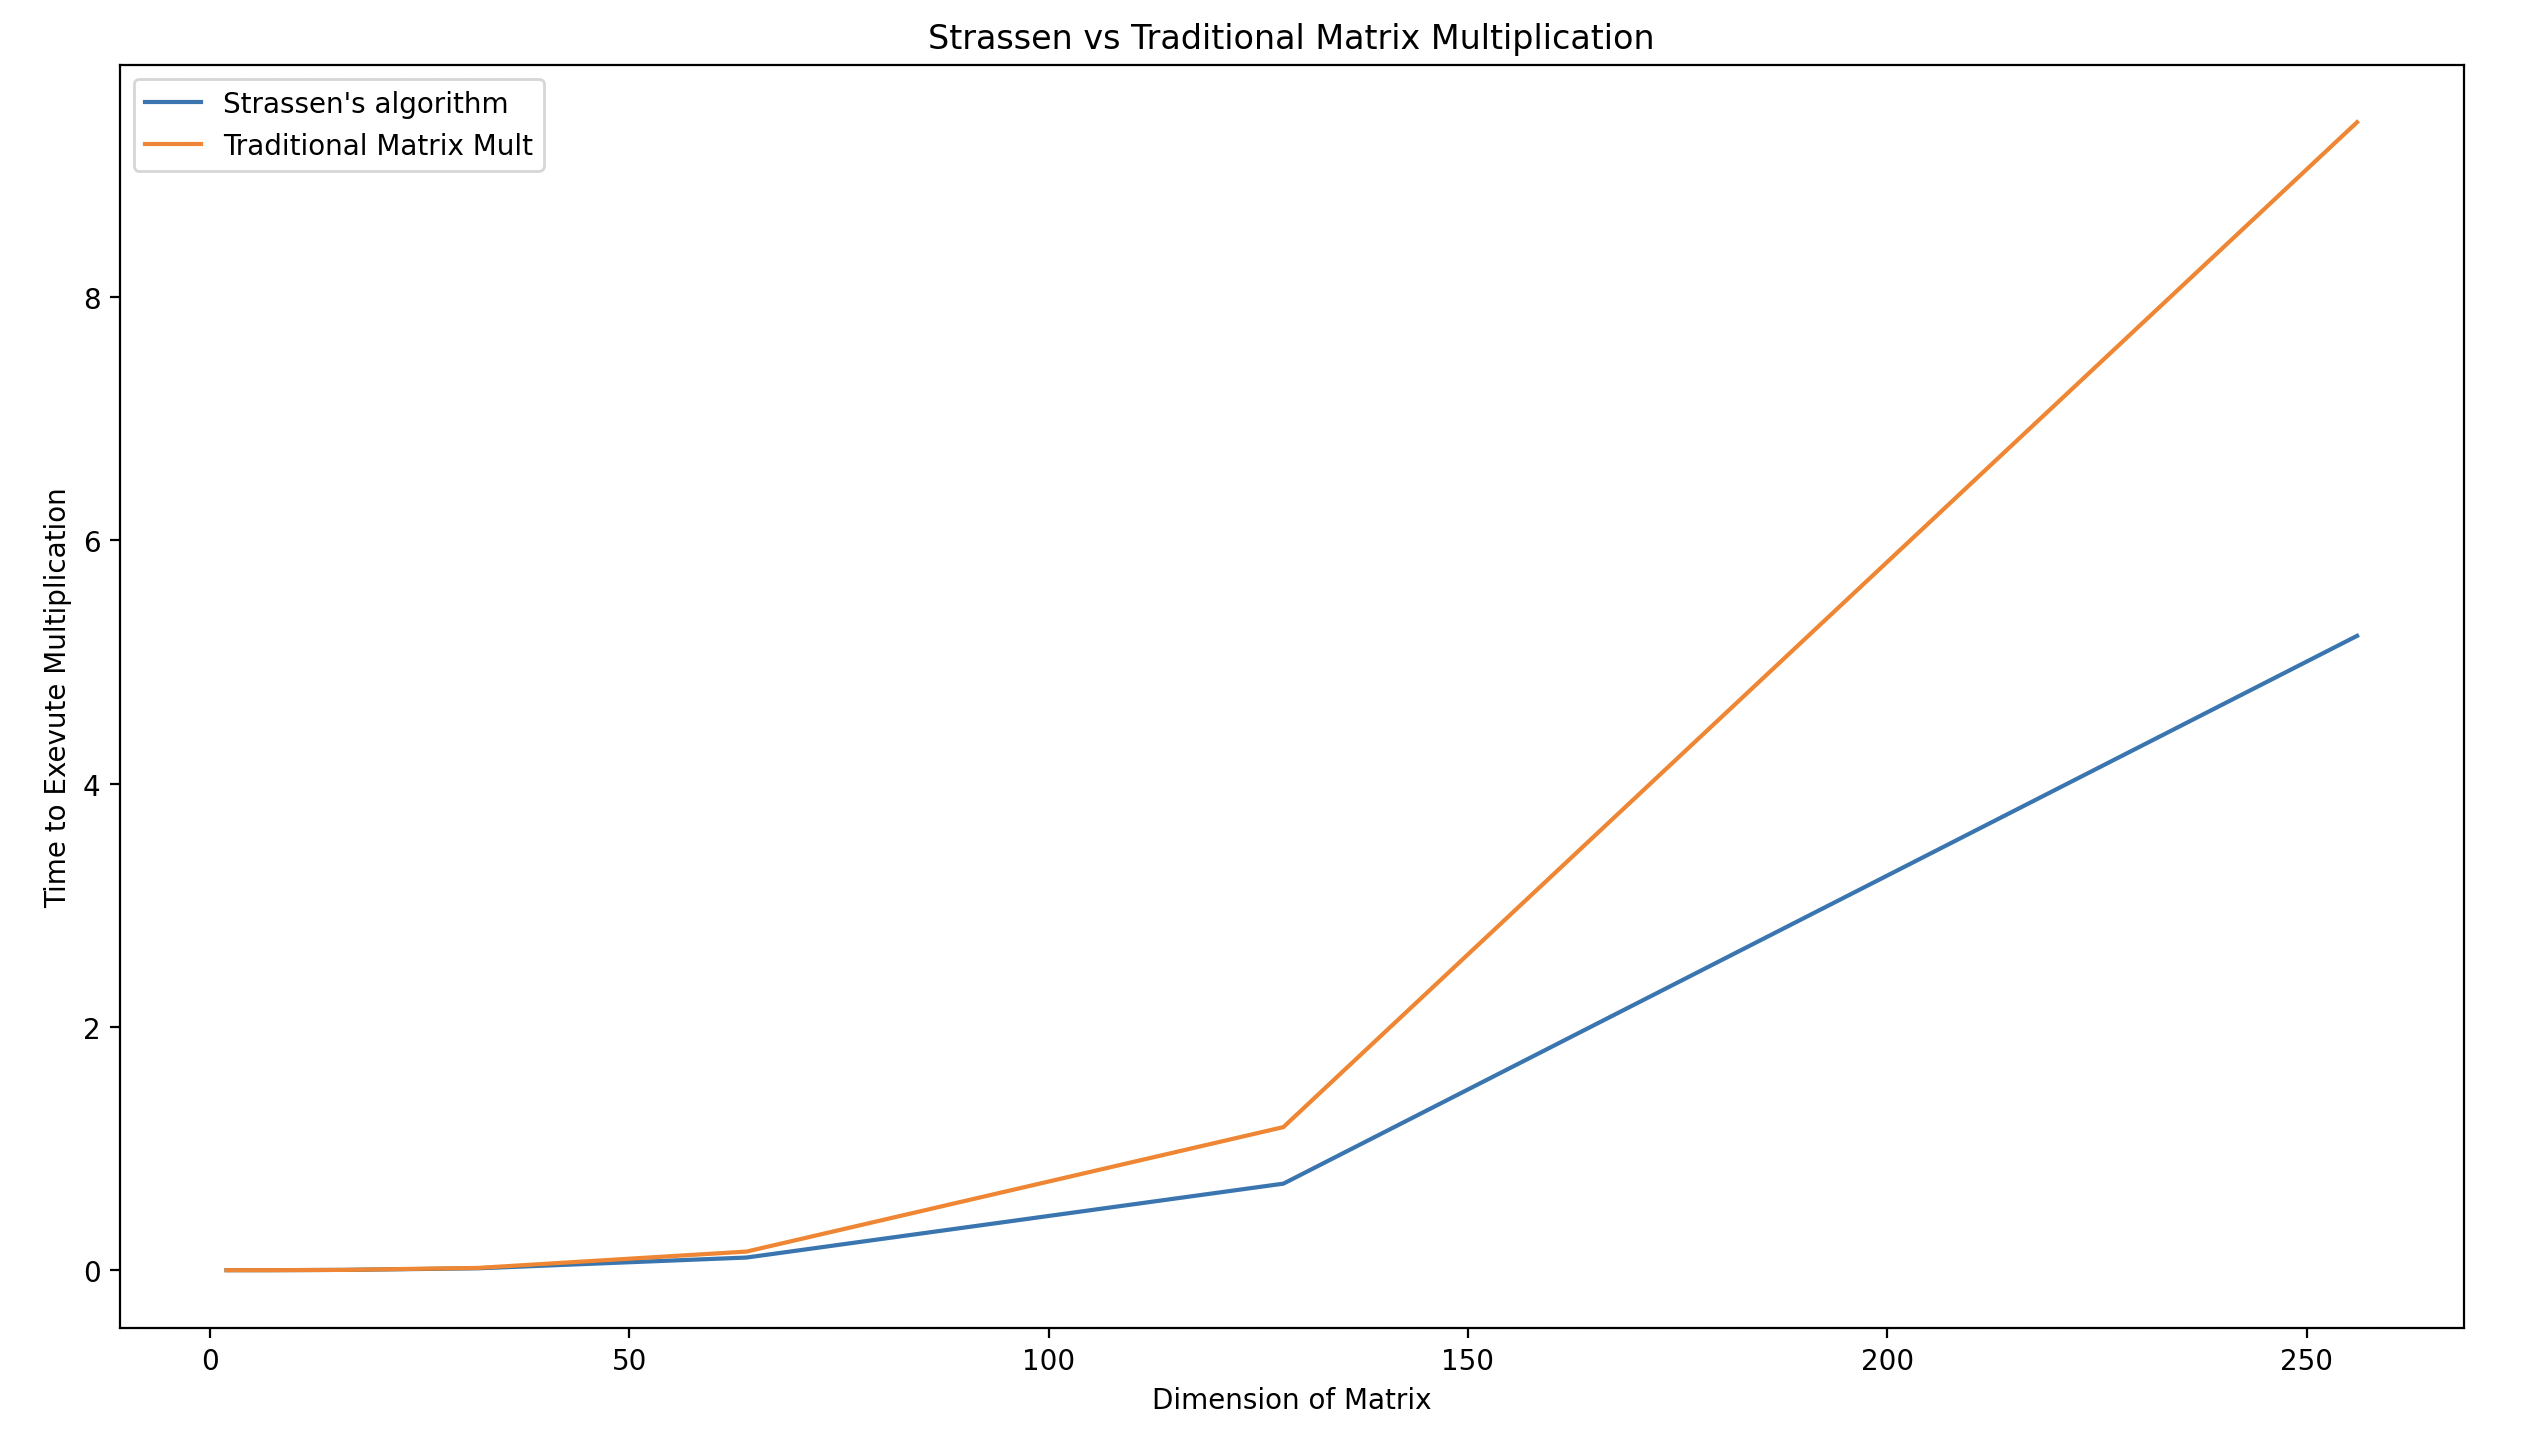
\includegraphics[width=\textwidth]{graph4.png}
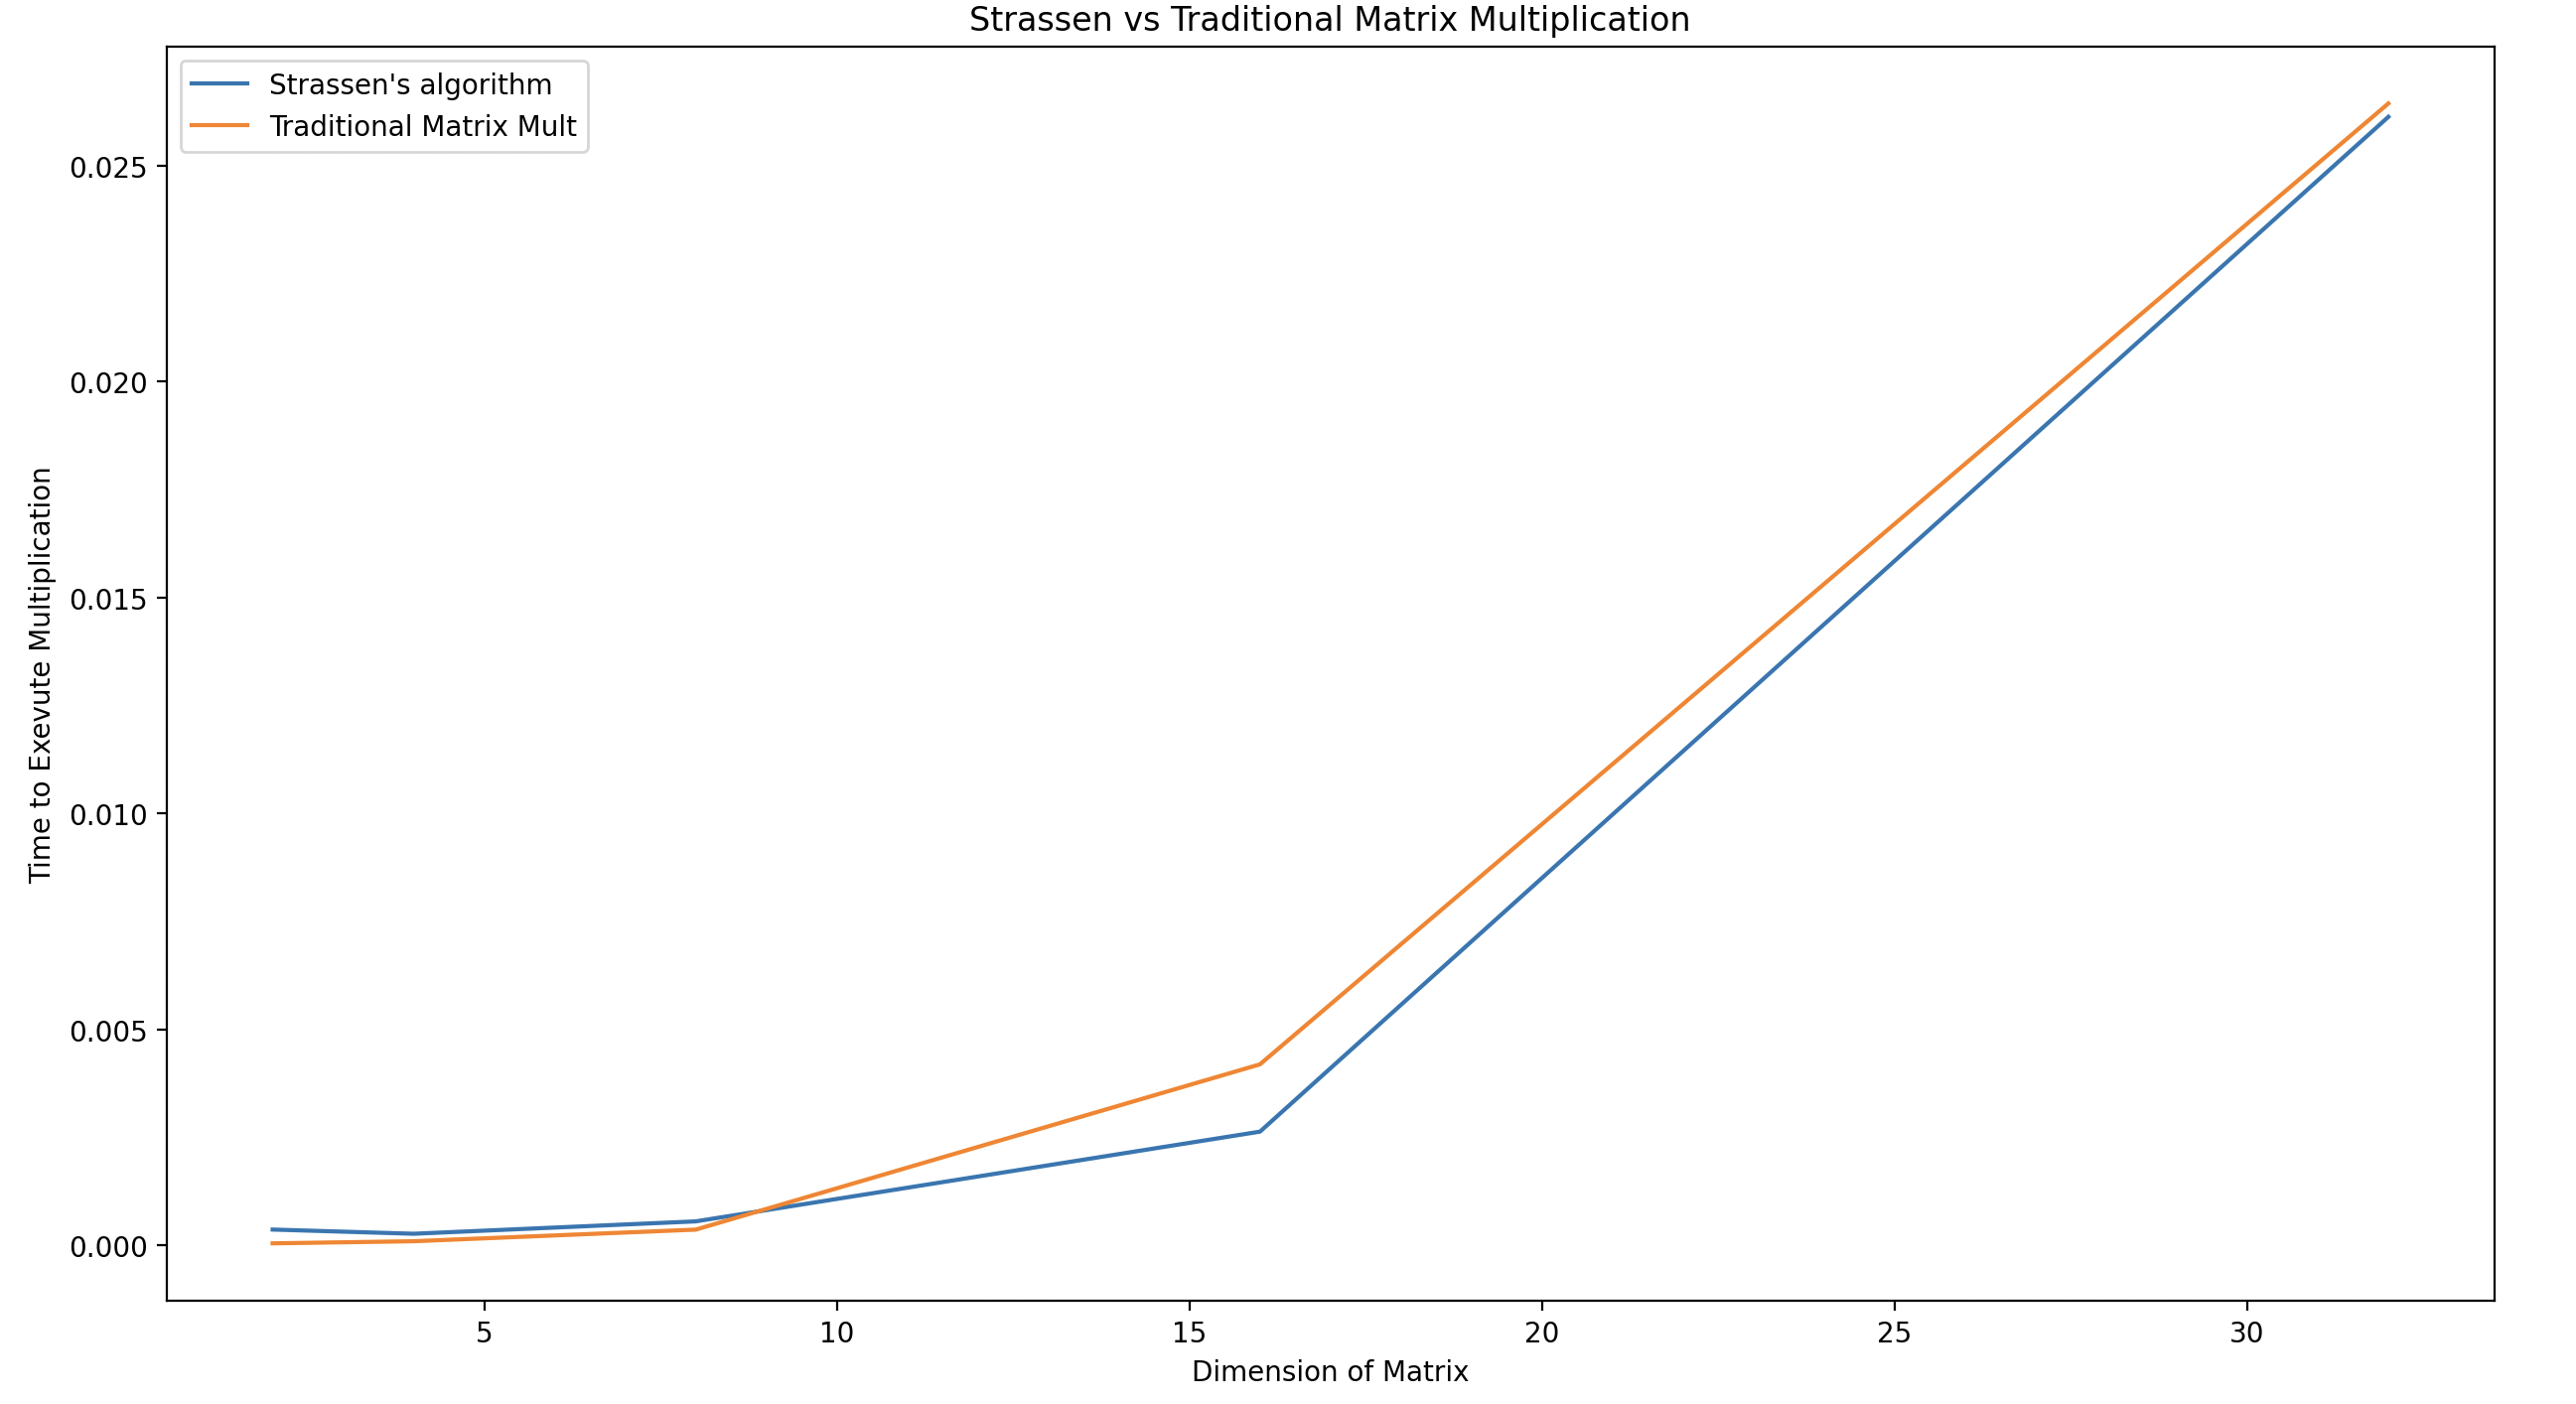
\includegraphics[width=\textwidth]{graph5.png} \\

This data matches my results from the first part of the experimental results. It seems that again, the two are very close for smaller dimensional matrices, but at n = 9, Strassen's seems to overtake the traditional matrix multiplication in terms of speed. This corroborates with all the data we've seen so far and makes sense. One way to optimize both algorithms would be to rely more heavily on NumPy's built in matrix multiplication algorithms such as the dot product. Doing this could lead to the cross over point being much higher. This is because python packages are typically written in C, which is a much faster language than python, so these packages are usually for faster than implementing the same algorithm in python. This could explain why our cross over point is relatively small.

\section{Section 3: Triangle in Random Graphs}

\end{document}
